
\subsubsection*{Flight Reservation (FR)}

In this example, we reuse the setting described in Section \ref{sec:intro}.
There are two types of agents: ticket sellers and ticket buyers. Ticket sellers are 
airlines which put up the air tickets for sale. Ticket buyers
are users who wants to travel from one city to another either on a direct
flight or by several hops. 
There are five cities ($a$ through $e$) 
and \figref{fig:flight} shows the flight connectivity map where 
an edge indicates that there is direct flight (in both directions) 
connecting two cities and the number on the edge is the price of the
flight. 
% For simplicity we ignore the flight times. 
In the seller program (Listing \ref{lst:tsell}), 
the ticket seller loops for several times, 
each time picks an edge randomly, 
and sells a ticket corresponding to that edge
(direction is also randomly selected). 
In the buyer program (Listing \ref{lst:tbuy}), 
every traveler (buyer) has exactly \$100 and tries to acquire enough tickets
that would fly him or her from $a$ to $e$ so long as the total price is 
less than \$100. In other words, $a\to b\to e$ 
and $a\to c\to d\to e$ are both possible routes.
{\tt fly()} is defined using pattern matching on parameters.
The base case is to arrive at the destination in the first fly, i.e.
{\tt fly(e, e, ...)} will evaluate to a symbol {\tt arrived} since 
the starting point is the destination. 
The recursive case is {\tt fly(a, e, ...)} will obtain unvisited neighbors and call {\tt try()}.
Note that using recursion with speculative nondeterminism is straightforward
as it is considered as a local computation and 
local computations are neither limited nor affected by our framework.

\begin{figure}[tb]
\centering
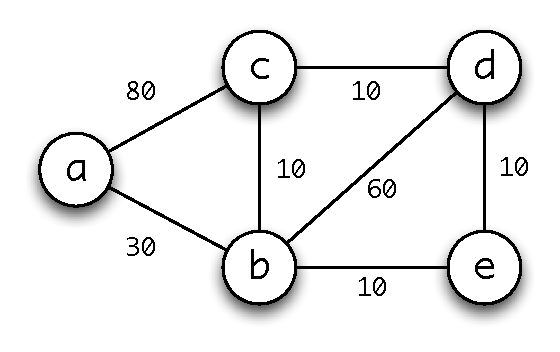
\epsfig{file=eps/flight-costs.eps,width=0.45\columnwidth}
\caption{Flight Map and Cost Between 5 Cities}
\label{fig:flight}
\end{figure}

\begin{figure}[tb]
\begin{lstlisting}[label=lst:tsell,caption=Ticket Seller's Agent. \texttt{[...]} denotes a list while \texttt{X[$i$]} is the $i$-th element of list \texttt{X}. \texttt{rand($m$)} returns a random integer between $0$ and $m$ (inclusive). \texttt{X.Y} denotes the concatenation of symbols so that \texttt{u.v} evaluates to \texttt{uv}.]
Ts = [[a,b,30],[a,c,80],[b,c,10],
      [b,d,60],[b,e,10],[c,d,10],[d,e,10]]
loop
  T = Ts[rand(6)]
  if rand(1) = 0
    |$\Out$|(ticket, T[0].T[1], T[2])
  else
    |$\Out$|(ticket, T[1].T[0], T[2])
|$\exit$|
\end{lstlisting}
\begin{lstlisting}[label=lst:tbuy,caption={Ticket Buyer's Agent. Both {\tt fly()} and {\tt try()} are defined using pattern matching on parameters. \texttt{[N:Ns]} denotes a list which has \texttt{N} as its head and \texttt{Ns} as its tail. Underscore (\texttt{\_}) matches anything in the context of pattern matching.}]
fly(X, X, Cash, V): arrived
fly(X, Y, Cash, V): Ns = unvisited_neighbors(X, V)
                    try(X, Ns, Y, Cash, V)

try(X, [N],    Y, Cash, V): buy(X, N, Y, Cash, V)
try(X, [N:Ns], Y, Cash, V): (buy(X, N, Y, Cash, V)
                            |$\oplus$|try(X, Ns, Y, Cash, V))
                            |$\cm$|

buy(X, N, Y, Cash, V):
  |$\In$|(ticket, X.N, |$\lambda x.x\le\texttt{Cash}$|) = (_, _, Cost)
  fly(N, Y, Cash - Cost, [N:V])

fly(a, e, 100, [a])
|$\exit$|
\end{lstlisting}
\vspace*{-5mm}
\end{figure}
